\documentclass[a4paper,10pt,twoside]{article}
\usepackage[polish]{babel}
\usepackage[utf8]{inputenc}
\usepackage[T1]{fontenc}
\usepackage{indentfirst}
\usepackage[top=2.5cm, bottom=2.5cm, left=2.5cm, right=2.5cm]{geometry}
\usepackage{graphicx}
\usepackage{amsmath}
\usepackage{booktabs}

\begin{document}

\begin{center}
\bgroup
\def\arraystretch{1.5}
\begin{tabular}{|c|c|c|c|c|c|}
	\hline
	EAIiIB & \multicolumn{2}{|c|}{Piotr Morawiecki, Tymoteusz Paszun} & Rok II & {Grupa 3a} & {Zespół 6} \\
	\hline
	\multicolumn{3}{|c|}{\begin{tabular}{c}Temat: Opracowanie danych pomiarowych \end{tabular}} & 
	\multicolumn{3}{|c|}{\begin{tabular}{c}Numer ćwiczenia: 0 \end{tabular}} \\
	\hline
	\begin{tabular}{@{}c@{}}Data wykonania:\\11.10.2017r.\end{tabular} & \begin{tabular}{@{}c@{}}Data oddania:\\18.10.2017r.\end{tabular} & 
	\begin{tabular}{c}Zwrot do poprawki:\\\phantom{data} \end{tabular} & \begin{tabular}{c}Data oddania:\\\phantom{data}\end{tabular} &
	\begin{tabular}{@{}c@{}}Data zaliczenia:\\\phantom{data}\end{tabular} & \begin{tabular}{c}Ocena:\\\phantom{ocena}\end{tabular} \\[4ex]
	\hline
\end{tabular}
\egroup
\end{center}

\section{Cel ćwiczenia}

Celem ćwiczenia jest zapoznanie się z metodami opracowania danych pomiarowych oraz szacowania niepewności pomiarów. Cel jest realizowany podczas próby wyznaczenia przyspieszenia grawitacyjnego Ziemi przy pomocy wahadła matematycznego.

\section{Wstęp teoretyczny - wahadło matematyczne}

Wahadło matematyczne to masa punktowa m zawieszona na nierozciągliwej i nieważkiej nici o długości l poruszająca się w jednorodnym polu grawitacyjnym. Podczas ćwiczenia użyjemy metalowego ciężarka zawieszonego na cienkiej lince, które stanowią dobre przyblizenie takiego układu.

Wprawiając wahadło w ruch poprzez wychylenie o niewielkie kąty $\theta$ możemy zastosować przybliżenie $\sin\theta\approx\theta$. W takim przypadku z uproszczonego równania ruchu wahadła otrzymamy zależność: $$T = 2\pi\sqrt{\frac{l}{g}}$$gdzie $T$ to okres drgań wahadła, $l$ to długość nici, a $g$ jest przyspieszeniem grawitacyjnym. Po przekształceniu równania otrzymujemy wzór na przyspieszenie grawitacyjne: $$g = \frac{4\pi^2l}{T^2}$$

\section{Opis doświadczenia}

\subsection{Stała długość wahadła}

W pierwszej części doświadczenia zebrane zostały pomiary czasów okresów wahadła dla stałej długości $l = 485mm$. Wahadło zostało wprawione w ruch jednocześnie z uruchomieniem stopera. Co dwadzieścia okresów ze stopera był odczytywany pomiar czasu od startu. Koniec miał miejsce po uzyskaniu dziesięciu odczytów (i wykonaniu przez wahadło dwustu okresów). Czas kolejnych dwudziesu okresów został wyznaczony na podstawie różnicy pomiędzy kolejnymi odczytami wskazań stopera.

Pomiar dla stałej długości został powtórzony mierząc czas co trzydzieści okresów - dokonano pięciu odczytów, do wykonania przez wahadło stupięćdziesięciu okresów.

\subsection{Zmienna długość wahadła}

W drugiej części doświadczenia zebrane zostały pomiary czasów okresów wahadła dla różnych długości. Wahadło było wprawiane w ruch jednocześnie z uruchomieniem stopera. Po wykonaniu przez wahadło dwudziestu okresów stoper był zatrzymywany, a wynik zapisywany. Po wykonaniu pomiaru długość wahadła została zwiększana i następował kolejny pomiar.

\section{Wyniki pomiarów}

\begin{table}[!htbp]
\caption{Pomiary dla wahadła o długości $l=485mm$, czas mierzony co 20 okresów}
\centering
\def\arraystretch{1.4}
\begin{tabular}{@{}rcccc@{}}
\\
\toprule
\begin{tabular}{@{}c@{}}Lp.\end{tabular} &
\begin{tabular}{@{}c@{}}Liczba okresów $k$\end{tabular} &
\begin{tabular}{@{}c@{}}Czas $t$ dla $k$ okresów [$s$]\end{tabular} &
\begin{tabular}{@{}c@{}}Czas $t'$ dla 20 okresów [$s$]\end{tabular} &
\begin{tabular}{@{}c@{}}Czas 1 okresu [$s$]\end{tabular}\\
\midrule
1  &  20   &  27,52   &  27,52  &  1,376  \\
2  &  40   &  62,36   &  34,84  &  1,742  \\
3  &  60   &  98,67   &  36,31  &  1,8155 \\
4  &  80   &  133,45  &  34,78  &  1,739  \\
5  &  100  &  168,08  &  34,63  &  1,7315 \\
6  &  120  &  202,58  &  34,5   &  1,725  \\
7  &  140  &  235,92  &  33,34  &  1,667  \\
8  &  160  &  275,92  &  40     &  2      \\
9  &  180  &  311,98  &  36,06  &  1,803  \\
10 &  200  &  349,08  &  37,1   &  1,855  \\
\bottomrule
\end{tabular}
\end{table}


\begin{table}[!htbp]
\caption{Pomiary dla wahadła o długości $l=485mm$, czas mierzony co 30 okresów}
\centering
\def\arraystretch{1.4}
\begin{tabular}{@{}rcccc@{}}
\\
\toprule
\begin{tabular}{@{}c@{}}Lp.\end{tabular} &
\begin{tabular}{@{}c@{}}Liczba okresów $k$\end{tabular} &
\begin{tabular}{@{}c@{}}Czas $t$ dla $k$ okresów [$s$]\end{tabular} &
\begin{tabular}{@{}c@{}}Czas $t'$ dla 30 okresów [$s$]\end{tabular} &
\begin{tabular}{@{}c@{}}Czas 1 okresu [$s$]\end{tabular}\\
\midrule
1  &  30   &  40,11   &  40,11  &  1,337  \\
2  &  60   &  90,39   &  50,28  &  1,676  \\
3  &  90   &  144,45  &  54,06  &  1,802  \\
4  &  120  &  193,17  &  48,72  &  1,624  \\
5  &  150  &  245,76  &  52,59  &  1,753  \\
\bottomrule
\end{tabular}
\end{table}


\begin{table}[!htbp]
\caption{Pomiary dla zmiennej długości wahadła}
\centering
\def\arraystretch{1.4}
\begin{tabular}{@{}rccrr@{}}
\\
\toprule
\begin{tabular}{@{}c@{}}Długość wahadła [$mm$]\end{tabular} &
\begin{tabular}{@{}c@{}}Czas 20 okresów [$s$]\end{tabular} &
\begin{tabular}{@{}c@{}}Czas 1 okresu [$s$]\end{tabular} &
\begin{tabular}{@{}c@{}}Wartość $g$\\~[$\frac{m}{s^2}$]\end{tabular} \\
\midrule
135  &  14,23  &  0,7115  &  10,52794716  \\
175  &  16,1   &  0,805   &  10,66119838  \\
215  &  18,4   &  0,92    &  10,02818973  \\
255  &  19,09  &  0,9545  &  11,04963804  \\
295  &  20,56  &  1,028   &  11,02035344  \\
335  &  23     &  1,15    &  10,00020408  \\
375  &  24,81  &  1,2405  &  9,620496086  \\
415  &  25,59  &  1,2795  &  10,00753812  \\
455  &  26,75  &  1,3375  &  10,04115225  \\
485  &  27,73  &  1,3865  &  9,96005479   \\
\bottomrule
\end{tabular}
\end{table}

\newpage

\section{Opracowanie wyników}

\subsection{Zawartość błędów grubych}

1. Pomiary dla stałej długości wahadła wskazują na poważne błędy podczas wykonania doświadczenia. O ile wartość przyspieszenia grawitacyjnego wyznaczona na podstawie pierwszego odczytu daje wynik zbliżony do spodziewanej wartości tabelarycznej, tak już kolejne różnią się od niej znacznie. Taką samą tendencję można zaobserwować dla powtórzonych pomiarów.

2. Wartości przyspieszenia grawitacyjnego dla pomiarów dla zmiennej długości wahadła wskazują, że dla wartości $l=255mm$ oraz $l=295mm$ mógł nastąpić błąd w liczeniu ilości okresów.

\subsection{Niepewność pomiaru okresu}

Niepewność pomiaru okresu obliczamy metodą typu A, czyli jako estymator odchylenia standardowego wartości średniej:

$$u(T)\equiv s_{\overline{T}} = \sqrt{\frac{\sum{(T_i-\overline{T})^2}}{n(n-1)}} = \sqrt{\frac{\sum{(T_i-1,65s)^2}}{90}} = 0,31 [s] $$

\subsection{Niepewność pomiaru długości wahadła}
Pomiar długości wahadła był wykonywany za pomocą linijki z działką o dokładności $1mm$, więc:
$$u(l)=1 [mm]$$

\subsection{Obliczenie przyspieszenia grawitacyjnego Ziemi}

$$g = \frac{4\pi^2l}{T^2} = 7,02 \frac{m}{s^2}$$

\subsection{Niepewność złożona}

$$u_c(g)=\sqrt{\frac{64\pi^4 l^2}{T^6}u(T)^2+\frac{16\pi^4}{T^4}u(l)^2} =  0,37 [\frac{m}{s^2}]$$

\subsection{Niepewność rozszerzona}

$$U_c(g) = k \cdot u_c(g) = 2 \cdot 0,37 [\frac{m}{s^2}] = 0,74 [\frac{m}{s^2}] $$

\subsection{Zgodność z wartością tabelaryczną}

Uzyskana wartość przyspieszenia grawitacyjnego $g = 7,02 \frac{m}{s^2}$ nie jest zgodna (w granicach wartości niepewności rozszerzonej) z wartością tabelaryczną $g_{krk} = 9,811 \frac{m}{s^2}$:

$$\vert g - g_{krk} \vert = 2,791$$

\newpage

\subsection{Wykresy}

\begin{figure}[!htp]
\centerline{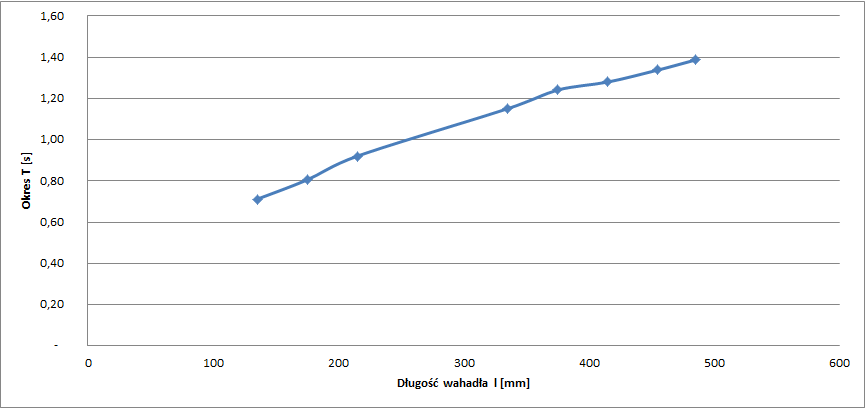
\includegraphics[scale=1]{wykres1.png}}
\caption{Wykres zależnosci długości okresu od długości wahadła}
\label{fig:tl}
\end{figure}

\begin{figure}[!htp]
\centerline{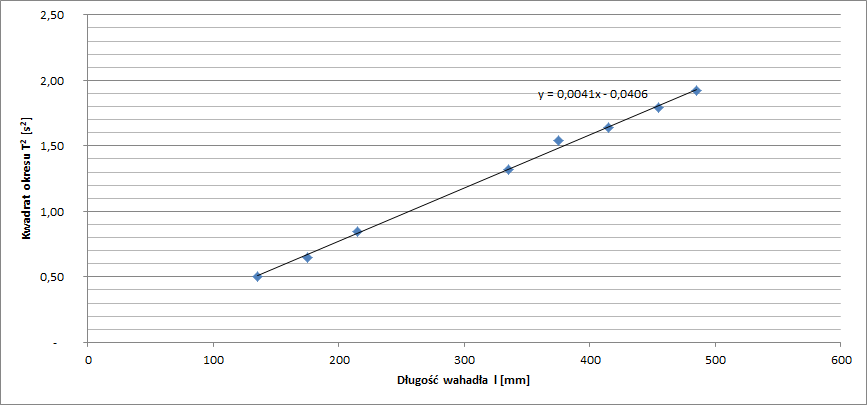
\includegraphics[scale=1]{wykres2.png}}
\caption{Wykres zależnosci kwadratu długości okresu od długości wahadła}
\label{fig:ttl}
\end{figure}

\subsection{Regresja liniowa metodą najmniejszych kwadratów}

Do punktów doswiadczalnych dopasowano prostą $y = a x$ metodą najmniejszych kwadratów:

$$ a = \frac{\sum l_i T_i}{\sum l_i^2} = 3,906510974$$

Wartość przyspieszenia grawitacyjnego jest określona wzorem:

$$ g = \frac{4 \pi^2}{a} = 10,10579974 \frac{m}{s^2} $$

Wartość niepewności współczynnika nachylenia $a$:

$$ u(a) = \sqrt{ \frac{S^2}{(n - 1)\sum x_i^2} } = 0,05558272514 [\frac{s^2}{m}]$$

Wartość niepewności przyspieszenia grawitacyjnego $g$:

$$ u(g) = \vert - \frac{4 \pi^2}{a^2} u(a) \vert = 0,1437876134 [\frac{m}{s^2}]$$

$$ U(g) = k \cdot u(g) = 0,2875752268 [\frac{m}{s^2}]$$

Uzyskana wartość nie mieści się w niepewności zwykłej, ani rozszerzonej:

$$ \vert g - g_{krk} \vert = 10,10579974 \frac{m}{s^2} - 9,811 \frac{m}{s^2} = 0,29479974 $$

\section{Wnioski}



\end{document}
